	\chapter{Intermediate Language}
	\label{chap:cep}
	
	Regular languages are widely used in computer science as they can be represented efficiently by finite state machines.		
	In our research according to \citep{davidi} I found out, that using regular expressions with timing extensions and parameters we are able to express the temporal patterns of VIATRA-CEP.
	Since regular expressions are widely used by the engineers and finite state automata provide clear semantics they are a good candidate as an intermediate language.
	
	First we overview formalisms from the literature, and suggest parametric timed region automaton as an intermediate formalism.
	As many of the high level specification languages like VEPL and Sequence charts can be characterized with the help of regular languages,
	this was the motivation behind our research.% Our findings are based on \citep{dicep}.
	
	We are going to introduce every step through an example: 
	We will specify a runtime verification component (also known as monitor) which will be in accepting state if the system is violating the rules of the two phase lock algorithm extended with a timeout.
	This can be considered as a runtime verification component of such system. This example is based on the File System example of paper \citep{marq}.
	
	In the two phase locking algorithm there are three rules to be held :
	\begin{enumerate}
		\item Resources must be allocated in a previously defined sequence (this sequence is the same for all tasks).
		\item If a task releases a resource, it is not allowed to do any more allocations.
		\item The first phase must finish after 10 seconds, i.e.~the time between the first allocation and the first release must be less than 10 seconds\footnote{We could use a better example such as ``A resource can not be in allocated state for more than 10 sec'', but this would make the example really complex.}. 
	\end{enumerate}
	
	Since this example uses resources, their behavior is defined as following:
	Each resource can be allocated once before every release, and can be released once before every allocation.
		
	\section{Overview of Formalisms}
	
	%\todo{The figure needs the not region automaton}
	%
	%\begin{figure}[h]
	%	\centering
	%	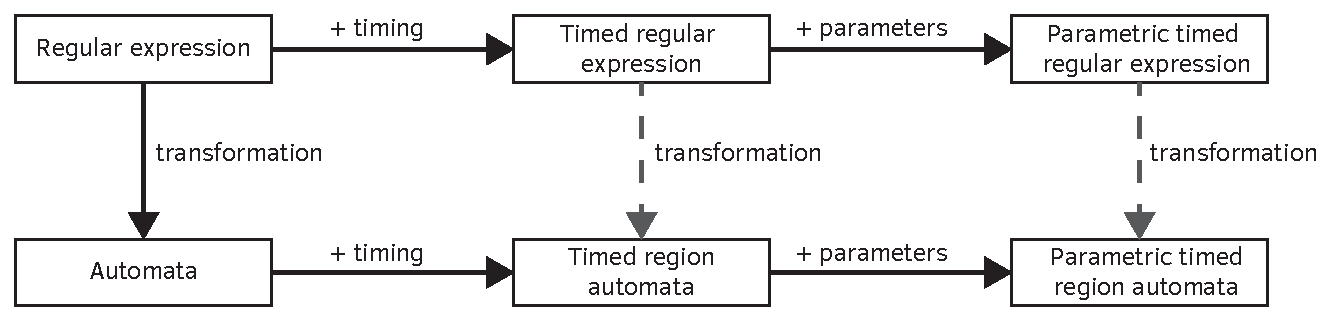
\includegraphics[width=0.95\linewidth]{figures/chapter_4/folyamatabra}
	%	\caption{Overview of the formalisms \redraw}
	%	\label{fig:cep:folyamatabra}
	%\end{figure}
	
	\begin{figure}[h]
			\begin{tikzpicture}[ edge/.style={thick, ->}]
			\small{
				\matrix (m) [matrix of nodes, nodes={rect,text width=0.2\linewidth, anchor=center 
				,  minimum height=4.25em}, row sep=3em, column sep=5em]
				{
					Regular\linebreak{}Expression &  Timed Regular Expression & Parametric Timed Regular Expression \\
					Nondeterministic Event Automaton &  Nondeterministic Timeout Region Event Automaton &  Parametric Timeout Region Event Automaton \\
					 Deterministic Event Automaton & Nondeterministic Timeout Event Automaton &  Parametric Timeout Event Automaton \\
				};
			}
			\footnotesize{
			\draw[edge](m-1-1) -- (m-1-2) node[midway, above, align=center]{+timing};
			\draw[edge](m-1-2) -- (m-1-3) node[midway, above, align=center]{+parameters};
			%
			\draw[edge](m-2-1) -- (m-2-2) node[midway, above, align=center]{+timing};
			\draw[edge](m-2-1.south east) -- (m-3-2.north west) node[midway, above, sloped, align=center]{+timing};
			%
			\draw[edge] (m-2-2) -- (m-2-3)  node[midway, above, align=center]{+parameters};
			\draw[edge] (m-3-2) -- (m-3-3) node[midway, above, align=center]{+parameters};
			%
			\draw[edge] (m-1-1) -- (m-2-1)  node[midway, right, align=center]{transformation};
			\draw[edge] (m-2-1) -- (m-3-1) node[midway, right, align=center]{transformation};
			%
			\draw[edge] (m-1-2) -- (m-2-2) node[midway, right, align=center]{transformation};
			\draw[edge] (m-2-2) -- (m-3-2) node[midway, right, align=center]{transformation};
			%
			\draw[edge] (m-1-3) -- (m-2-3) node[midway, right, align=center]{transformation};
			\draw[edge] (m-2-3) -- (m-3-3) node[midway, right, align=center]{transformation};
			}
			\end{tikzpicture}
		\caption{Overview of the formalisms }
		\label{fig:cep:folyamatabra}
	
	\end{figure}%
	
	The used formalisms and their relations are show on \cref{fig:cep:folyamatabra}.
	The vertical arrows show that for each regular expression an automaton can be constructed with a transformation, which accepts the language specified with the regular expression.
	The horizontal arrows show that each formalism can be extended with the required properties; timing and parameters respectively.
	Note that even the Deterministic Event Automaton could be extended with Timing, and a formalism could be constructed for it, however there are no known algorithms to construct a Deterministic Timed Automaton.
		
	\section{Regular Languages}
	
		Regular Languages are commonly used both in the industry and in the academic researches as they commonly serve as a domain specific language.
		Most of their properties which are interesting from the academic point of view can be analyzed and decided, and they are simple enough to be used in industrial projects to ease up the description of something which does not require a more complex language.
	
		\subsection{Regular Expression}
		
			In this particular example, we need a language to describe event sequences. To do so, one of the most common formalism is regular expressions, where the alphabet $\Sigma$ is the set of possible events.
	
			
			\begin{dfn}
				\label{dfn:cep:re}
				Regular Expressions over an alphabet $\Sigma$ (also referred to as $\Sigma$-expressions)
				are defined using the following families of rules.
				\begin{enumerate}
					\item $a$ for every letter $a \in \Sigma$ and the special symbol $\varepsilon$ are expressions.
					\item If $\varphi, \varphi_1, \varphi_2$ are $\Sigma$-expressions then %
						$ %
						\varphi_1 \varphi_2,
						\varphi_1 | \varphi_2,
						\varphi^\ast
						$ are $\Sigma$-expressions\citep{tre}.
				\end{enumerate}
			\end{dfn}
	
			The meaning of these operators:
			\begin{itemize}
				\item $\varphi_1 \varphi_2$: Sequence, $\varphi_2$ must occur after $\varphi_1$.
				\item $\varphi_1 | \varphi_2$: Choice, $\varphi_1$ or $\varphi_2$ must happen.
				\item $\varphi^\ast$: Closure (also known as Kleene-star), $\varphi$ can occur $n$ times, where $0 \leq n < \infty$
			\end{itemize}
			
	
			To illustrate the usage of the regular expressions in the two phase locking example, the behavior ``After a task has released a resource, it's not allowed to allocate again'' is described with the regular expression : $a (a)^* r (r)^* a $, where $a$ is short for allocation and $r$ is short for release.
	
	
		\subsection{Deterministic Finite Event Automaton}
			To accept regular expressions, the most common solution is to construct an automaton accepting the language generated by the regular expressions. Various  algorithms exist for the generation of deterministic finite automaton from regular expressions. \todo{Cite?}
			
			\begin{dfn}
				\label{dfn:cep:ea}
				A Deterministic Finite Event Automaton is a tuple $\langle Q,\Sigma,\delta,q_0, F \rangle$\citep{lam2006compilers} where: 
					\begin{itemize}
						\item $Q$ is a finite, nonempty set, representing the states of the automaton,
						\item $\Sigma$ is a finite, nonempty set, representing the event set of the automaton,
						\item $\delta$ is a subset of tuples $\langle Q \times \Sigma \times Q \rangle$,
							and the number of outgoing edges from each state for each event is only one 
							i.e.~$\forall s_0 \in Q$ and $\forall e_0 \in \Sigma$ : $|\langle s_0, e_0, s_1 \rangle| = 1$, where $s_1 \in Q$. Nondeterminism is not allowed,
						\item $q_0 \in Q$ the initial state,
						\item $F \subseteq Q$ the set of the accepting states.
					\end{itemize}	
			\end{dfn}
		
			\begin{dfn}
				\label{dfn:cep:ea:inputseq}
				An input sequence for a Deterministic Finite Automaton is $(e_1, e_2, \dots, e_n )$, where $\forall i : e_i \in \Sigma$, i.e.~a sequence of events.
			\end{dfn}
		
			\begin{dfn}
				\label{dfn:cep:ea:trace}
				A trace in an Deterministic Event Automaton is
				a sequence of states $(r_0, r_1, \dots, r_m)$, where $\forall i: r_i \in Q$,
				for the input sequence $(e_1, e_2, \dots, e_n)$ if:
				\begin{itemize}
					\item $r_0 = q_0$, i.e.~the first state of the trace is the initial state of the Automaton,
					\item If the automaton has a trace $(r_0,\dots,r_{i-1})$ for input sequence $(e_1,\dots,e_{j-1})$ then either
					\begin{itemize} 
						\item $\langle r_{i-1}, \varepsilon, r_i \rangle \in \delta$, or
						\item  $\langle r_{i-1}, e_j, r_i \rangle \in \delta$ is true,
					\end{itemize}
					\item the last $r_m$ state is reached by reading event $e_n$ (Or more precisely the after reading the last event $r_m$ is reachable using only
					$\varepsilon$-transitions)
				\end{itemize}
				A trace is accepting if $r_n \in F$.
			\end{dfn}
		
			\begin{dfn}
				\label{dfn:cep:ea:accepting}
				An event automaton accepts an input sequence if exists an accepting trace for the input sequence.
			\end{dfn}
		
			\begin{dfn}
				\label{dfn:cep:ea:token}
				A token in a Nondeterministic Finite Event Automaton a set of the active states.
			\end{dfn}
			
			Just to illustrate the operation of the Finite Automata we can use a token assigned to the active state.
	
			The semantics is illustrated as follows. 
			\begin{itemize}
				\item At initialization the token is at the initial state $f_0$.
				\item When receiving input $e$, where $e \in \Sigma$, if the token is on state $s$ the next state will be $s'$ where
				$\delta \langle s,e,s' \rangle$.% For short, from now the notation $s \rightarrow s'$ will be used. 
				\item If the token enters state $s'$ where $s' \in F$ then the input sequence is accepted. 			
			\end{itemize}
	
	
			The regular expression of the example can be compiled to the event automaton of~\cref{fig:cep:fa}. 
	
			Note that the automaton only accepts the incorrect traces as our complex event processing framework allows to define reactions when the automaton enters an acceptor state.
			
			\begin{figure}[h]
			\centering
			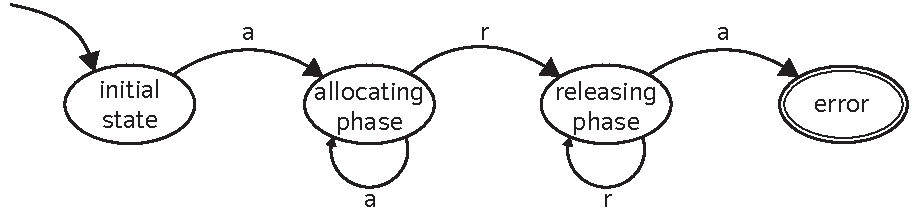
\includegraphics[width=0.7\linewidth]{figures/chapter_4/allocating_simple}
			\caption{Event automaton of the two phase locking example \redraw}
			\label{fig:cep:fa}
			\end{figure}
		
		\subsection{Nondeterministic Finite Event Automaton}
		
		\begin{dfn}	
			\label{dfn:cep:nea}
			A Nondeterministic Finite Event Automaton is a tuple $\langle Q,\Sigma',\delta,q_0, F \rangle$, where:
			\begin{itemize}
				\item $Q, q_0$, and $F$ are the same as in \cref{dfn:cep:ea},
				\item $\Sigma'$ is $\Sigma \cup \varepsilon$, where $\Sigma$ is the same as in \cref{dfn:cep:ea}
				\item $\delta$ is a subset of tuples $\langle Q \times \Sigma' \times Q \rangle$.
				Note that there could be more than one transition for one state with the same event.
			\end{itemize}
		\end{dfn}
	
		\begin{dfn}
			\label{dfn:cep:nea:trace}
			A trace in an Deterministic Event Automaton is
			a sequence of states $(r_0, r_1, \dots, r_n)$, where $\forall i: r_i \in Q$,
			for the input sequence $(e_1, e_2, \dots, e_n)$ if:
			\begin{itemize}
				\item$r_0 = q_0$, i.e.~the first state of the trace is the initial state of the Automaton,
				\item $\forall i \in (1,\dots,n-1): \langle r_i, e_{i+1}, r_{i+1} \rangle \in \delta$ i.e.~exists a transition between state $r_i$ and $r_{i+1}$ with the label of the $e_{i+1}$ according event.	
				\item The last $r_n$ is reached after reading the entire input sequence.	
			\end{itemize}
			A trace is accepting if $r_n \in F$.
		\end{dfn}
			
		\begin{dfn}
			\label{dfn:cep:nea:accepting}
			An event automaton accepts an input sequence if exists an accepting trace for the input sequence.
		\end{dfn}
		
		\begin{dfn}
			\label{dfn:cep:nea:token}
			A token in a Deterministic Finite Event Automaton is the active state.
		\end{dfn}
		
		\subsection{Transformation from Regular Expression to Deterministic Finite Automaton}
			The transformation of simple (not timed and parametric) regular expressions are well known in the current literature. The various algorithms were investigated and a chosen algorithm from \citep{lam2006compilers} is implemented.
	
			
			\subsubsection{Transformation from Regular Expression to Nondeterministic Automaton with $\bm{\varepsilon}$ transitions}
			\label{section:re2nfa}
			First the regular expression is transformed to a nondeterministic automaton with recursive rules for each operator
			\begin{itemize}
				\item The automaton corresponds to a simple event is constructed as an initial state and an acceptor state with one transition between them, which has the label of the event, as shown on \cref{fig:cep:nfaevent}. Note that this is the only non-recursive rule, as the concrete syntax tree's leaves are always Events, therefore this is where the recursion always stops.\todo{There is a better terminology for ``algorithm stops'' :D}
				\item The sequence of two expressions are compiled in two steps, first the two subexpressions are compiled into one automaton each. After that we merge the acceptors states of the first automaton with the initial state of the second automaton, i.e.~remove the acceptor flag from the first automaton's acceptor states, and add every outgoing transition of the second automaton's initial state to the first automatons acceptor states, as shown on \cref{fig:cep:nfasequence}
				\item A choice can be compiled in two steps. First the two subexpressions are compiled into one automaton each. In the second step we create one new initial state, and create a two $\varepsilon$-transition from the new initial state to the two subexpression's compiled automata's initial state. After that we create one $\varepsilon$-transition from their acceptor states to a newly created acceptor state. The result's initial state will be the newly created state and the result's only acceptor state will be the newly created one, as shown on \cref{fig:cep:nfachoice}
				\item A closure can also be compiled in two steps, first the internal expression has to be compiled to the automaton and a new initial and acceptor state has to be constructed. Then four $\varepsilon$ transition needs to be added:
				\begin{enumerate}
					\item From the compiled automaton's acceptor state to it's initial state,
					\item From the new initial state to the subexpression's initial state,
					\item From the subexpression's acceptor state to the new acceptor state,
					\item From the new initial state to the new acceptor state.
				\end{enumerate}
			\end{itemize}
		
			\todo{Missing the AND, probably just don't tell the reader about it?}
			
			\begin{figure}[h]
				\centering
				\begin{tikzpicture}[
				node distance=1cm and 2cm,
				edge/.style={->}
				]
					\node[state,initial] (initial) {$i$};
					\node[state,accepting, right=of initial] (final) {$f$};
					\draw[edge](initial) -- (final) node[midway, above, align=center]{$a$};
				\end{tikzpicture}
				\caption{Constructed NFA from the simple event $a$}
				\label{fig:cep:nfaevent}
			\end{figure}
		
			\begin{figure}[h]
				\centering
				\begin{tikzpicture}[
					edge/.style={->}
					]
					\node[state] (initial) {$i$};
					\node[right=of initial] (nt) {$N(t)$};
					\node[state, right=of nt] (common) {};
					\node[right=of common] (ns) {$N(s)$};
					\node[state,accepting, right=of ns] (final) {$f$};
					\node[draw, ellipse, initial, inner xsep=-3mm, fit=(initial) (nt) (common)] (left elipsis) {};
					\node[draw, ellipse, inner xsep=-3mm, fit=(common) (ns) (final)] (right elipsis) {};
				\end{tikzpicture}
				\caption{Constructed NFA from the sequence $N(s)\;N(t)$}
				\label{fig:cep:nfasequence}
			\end{figure}
			
			\begin{figure}[h]
			\centering
			\begin{tikzpicture}[
				edge/.style={->}
				]
				\node[state, initial] (initial) {$i$};
				%
				\node[state, above right=of initial] (nti) {};
				\node[right=of nti] (nt) {$N(t)$};
				\node[state, right=of nt] (ntf) {};
				\node[draw, ellipse, inner xsep=-3mm, fit = (nti) (nt) (ntf)] {};
				%
				\node[state, below right=of initial] (nsi) {};
				\node[right=of nsi] (ns) {$N(s)$};
				\node[state, right=of ns] (nsf) {};
				\node[draw, ellipse, inner xsep=-3mm, fit = (nsi) (ns) (nsf)] {};
				
				\node[state, accepting, above right=of nsf] (final) {$f$};
				
				\draw[edge] (initial) -- (nti) node[midway, above, sloped, align=center]{$\varepsilon$};
				\draw[edge] (initial) -- (nsi) node[midway, above, sloped, align=center]{$\varepsilon$};
				
				\draw[edge] (ntf) -- (final) node[midway, above, sloped, align=center]{$\varepsilon$};
				\draw[edge] (nsf) -- (final) node[midway, above, sloped, align=center]{$\varepsilon$};
				
			\end{tikzpicture}
			\caption{Constructed NFA from the choice $N(s)|N(t)$}
			\label{fig:cep:nfachoice}
		\end{figure}
			
			\begin{figure}[h]
				\centering
				\begin{tikzpicture}[
				edge/.style={->}, auto
				]
				\node[state, initial] (initial) {$i$};
				%
				\node[state, right=of initial] (nsi) {};
				\node[right=of nsi] (ns) {$N(s)$};
				\node[state, right=of ns] (nsf) {};
				\node[draw, ellipse, inner xsep=-3mm, fit = (nsi) (ns) (nsf)] {};
				%
				\node[state, accepting, right=of nsf] (final) {$f$};
				\path[->]
				(initial) edge node[near start] {$\varepsilon$}  (nsi)
				(nsf)     edge node[near end] {$\varepsilon$}                (final)  
				(nsf)     edge[bend left = 75] node {$\varepsilon$} (nsi)    
				(initial) edge[bend left = 60]  node {$\varepsilon$} (final) ;
				
				\end{tikzpicture}
				\caption{Constructed NFA from the closure $N(s)^*$}
				\label{fig:cep:nfasterisk}
			\end{figure}
			
	
			\subsubsection{Transformation from Nondeterministic Automaton to Deterministic Automaton}
			
					\begin{algorithm}
				\SetAlgoLined
				\SetKwInOut{Input}{input}\SetKwInOut{Output}{output}
				\Input{An NFA $N$}
				\Output{A DFA $D$ accepting the same language as $N$}
				initially, $\varepsilon$-closure($s_0$) is the only state in $\mathit{Dstates}$, and it is unmarked\;
				\While{there is an unmarked state $T$ in $\mathit{Dstates}$}{
					mark $T$\;
					\ForEach{input symbol $a$}{
						$U = $ $\varepsilon$-closure(move($T,a$))\;
						\If{$U$ is not in $\mathit{Dstates}$}{
							Add $U$ as an unmarked state to $\mathit{Dstates}$\;
						}
						$\mathit{Dtran}[T,a] = U$ \;
					}
				}
				\caption{The subset construction of a DFA from an NFA}
				\label{alg:cep:subset}
			\end{algorithm}
			
			\begin{algorithm}
				\SetAlgoLined
				\SetKwInOut{Input}{input}\SetKwInOut{Output}{output}
				\Input{A set of states $T$}
				\Output{A set of states $\varepsilon$-closure($T$)}
				push all states of $T$ onto $\mathit{stack}$\;
				initialize $\varepsilon$-closure($T$) to $T$\;
				\While{$\mathit{stack}$ is not empty}{
					pop $t$ from the $\mathit{stack}$ \;
					\ForEach{state $u$ with an edge from $t$ to $u$ labeled $\varepsilon$}{
						\If{$u$ is not in $\varepsilon$-closure($T$)}{
							Add $u$ to $\varepsilon$-closure($T$)\;
							push $u$ onto $\mathit{stack}$ \;
						}
					}
				}
				\caption{Computing $\varepsilon$-closure($T$)}
				\label{alg:cep:eclosure}
			\end{algorithm}
			
			The algorithm is introduced on \cref{alg:cep:subset}.
			The algorithm constructs a transition table $\mathit{Dtran}$ for $D$. Each state of $D$ is a set of NFA states, and we construct $\mathit{Dtran}$ so $D$ will simulate ``in parallel'' all possible moves $N$ can make on a given input trace. Our first problem is to deal with $\varepsilon$-transitions of $N$ properly.
	
			Move($T,a$) is the set of states of the NFA which there is a transition on input symbol $a$ from some state in $T$.
			
			The algorithm for calculating the $\varepsilon$-closure is shown on \cref{alg:cep:eclosure}.
			
		\section{Timed Regular Languages}	
		
		Timed Regular Languages are an extension over the Regular Languages to express timed properties.
		These timed properties are common in most of the usecases as many system has timed behavior which can be described using Timed Regular Languages.
		
			\subsection{Timeout Regular Expression}
		
			Using the previously defined semantics timed properties can not be expressed, but regular expressions can be extended to a formalism which can do so: the timeout regular expressions.
			
			\begin{dfn}
				\label{dfn:cep:tre}
				Timeout Regular Expressions over an alphabet $\Sigma$ (also referred to as $\Sigma$-expressions)
				are defined using the following rules.
				\begin{enumerate}
					\item $a$ for every letter $a \in \Sigma$ and the special symbol $\varepsilon$ are expressions.
					\item If $\varphi, \varphi_1, \varphi_2$ are $\Sigma$-expressions then %
						$ %
						\varphi_1 \; \varphi_2,
						\varphi_1 | \varphi_2,
						\varphi^\ast,$ and 
						$\langle \varphi \rangle_I$, 
						are $\Sigma$-expressions, where $I$ is an positive real number for timeout. % \citep{tre}
				\end{enumerate}
			\end{dfn}
	
	
			The new operator is $\langle \varphi \rangle_I$ which means, that the whole $\varphi$ has to be observed within the given time.	
			The implementation and algorithmization with intervals instead of timeouts as in \citep{tre} are considered future work.
	
			With the timed regular expression formalism the example can be extended with timing, and adding the concept timeout becomes possible.
			The new expression will be: $(a \; (a)^\ast \; r \; (r)^\ast \; a)|( \langle a \; (a)^\ast \; r \rangle_{10 s})$
			
			\subsection{Timeout Region Automaton}
			
			Timeout Region Automaton is introduced as an intermediate step between the Timeout Regular Expression and the Timeout Automaton as it is a step closer to the regular expression.
			However the Timeout Region Automaton has the same expressive power as the Timeout Regular Expression the more general and better known Timeout Automaton is more expressive.
			If in the future for some use cases the Regular Expression lacks the required expressiveness then the Timeout Automata can be used as an intermediate language as well.
			
			We add a syntactic sugar to ease the compilation of high level languages to this intermediate language.
			Using timed regions in our automaton language has the same motivation as the application of regions in state chart formalisms.
			
			From now on, the notation $\mathit{Reg}$ will be used for regions, which is a set of states, i.e.~$\mathit{Reg}~\subseteq~Q$
			
			
			\begin{dfn}
				\label{dfn:cep:trea}
				A Timeout Region Event Automaton is a tuple $\langle Q,\Sigma,\delta,q_0, F, t, T \rangle$ where
				\begin{itemize}
					\item $Q, q_0,$and $F$ are the same as in \cref{dfn:cep:nea},
					\item $\Sigma$ is the same as $\Sigma'$ in \cref{dfn:cep:nea}, 
					
					\item $T$ is a set of tuples $\langle \mathit{Reg}, \RR \rangle$ i.e.~a set of timeout clock variables for a set of states,
					\item and $\delta$ is the union of discrete and timed transitions i.e.~$\delta_t \cup \delta_d$ where
					\begin{itemize}
						\item $\delta_d$ is the same as $\delta$ in \cref{dfn:cep:nea},
						\item and $\delta_t$ represents timed transitions and defined as the set of tuples $\langle \mathit{Reg} , \mathbb{R} , Q \rangle$, i.e.~a tuple which represents a timed region, the value of the maximum time elapsed
					\end{itemize}
					
				\end{itemize}
			\end{dfn}
			
	%		WTF: \linebreak the set of which have outgoing timed transitions i.e.~$ \forall R_i \in \mathit{Reg}, \exists t, \exists q  \subseteq \delta_t \langle R_i, t, q \rangle$ 
			
			The semantics of the timed region automaton is defined as follows:
			$Q_t \subseteq Q$ is the set of states with outgoing timed transitions, 
			i.e.~$\forall q \in Q_t$ : $ q \in R $. 
			
			
			Let us use the following notations: 
			
			\begin{itemize}
				\item $s$ is the currently active state, and $s'$ is the next state according to $\delta$.		
				\item $r$ is the set of currently active regions, i.e.~$r \subseteq \mathit{Reg}$ where $\exists r_s : r_s \in r, s \in r_s $ 
				\item $r'$ is the set of regions the token enters, i.e.~$r \subseteq \mathit{Reg}$ where $\exists r_s :  r_s \in r, s' \in r_s $ 
				\item $r^+ \subseteq \mathit{Reg}$ is a set of timed regions the token has just entered, i.e.~$r^+ = r' \setminus r$ 
				\item $r^- \subseteq \mathit{Reg}$ is a set of timed regions the toke has just left i.e.~$r^- = r \setminus r'$
			\end{itemize}
			
			Rules  have to defined for the initialization of the automaton, entering states with timed outgoing transitions and we also define the general rules of changing states. 
			
			\begin{enumerate}
				\item Initialization Rule : At the initialization  of the automaton, we have to set all clock variables to $\infty$ 
				i.e.~$\forall t_i, \forall q_i, T \langle r_i, t_i \rangle, t_i \coloneqq \infty $, where $r_i \in R$
				
				\item Entering new timed region rule :
				If a token enters a new set of timed regions, 
				i.e.~$r^+ \neq \emptyset$, 
				the timers are set according to the timeouts, 
				i.e.~$\forall t_{\textit{timeout}} : t_{\textit{timeout}} \coloneqq t + t_i $ where $ r_t \in r^+, \exists q ,\delta_t\langle  r_t,t_i,q \rangle, T \langle r_t, t_{\textit{timeout}} \rangle$
				
				\item Firing Transition Rule: Choose an enabled transition from the set of enabled discrete or timed transitions. 
				There are two cases, the chosen transition is:
				\begin{enumerate}
					\item Discrete Transition: In case of $r^- = \emptyset$ than the execution of the transition is as in described formerly. 
					If the token exits a region i.e.~$r^- \neq \emptyset$, 
					then the following rule extends the firing rule of discrete transitions:
					$\forall t_s, \forall q_s$ in $ \delta_t \langle r_i, t_s, q_s \rangle$ where $r_i \in r^-$, the timer of the regions are invalidated i.e.~	$t_s \coloneqq \infty$
					\item Timed Transition: The transition with the minimal timeout value is selected, 
					i.e.~transition $\exists t_i, \exists s_i, \delta_t \langle r_i, t_i, s_i \rangle$ where $ r_i \in r$ and $t_{\textit{min}}$ is the minimum from all $t_i$,
					than the following rules apply:
					the global time is set $t \coloneqq t_{\textit{min}}$, 
					the local clocks the token just left are invalidated i.e.~
					$\forall t_s, \forall q_s$ in $ \delta_t \langle r_i, t_s, q_s \rangle$ where $r_i \in r^-$, the timer of the regions are invalidated i.e.~$t_s \coloneqq \infty$ 
					and move to the next state according to $\delta_t$.
				\end{enumerate}			
			\end{enumerate}
			
			
			We can generate from the expression $(a (a)^\ast r (r)^\ast a)|( \langle a (a)^\ast r \rangle_{t < 10 s})$ the automaton of~\cref{fig:cep:trea}.
			Note the additional timed region which contains the ``allocating phase'' state.
			
			\begin{figure}[h]
				\centering
				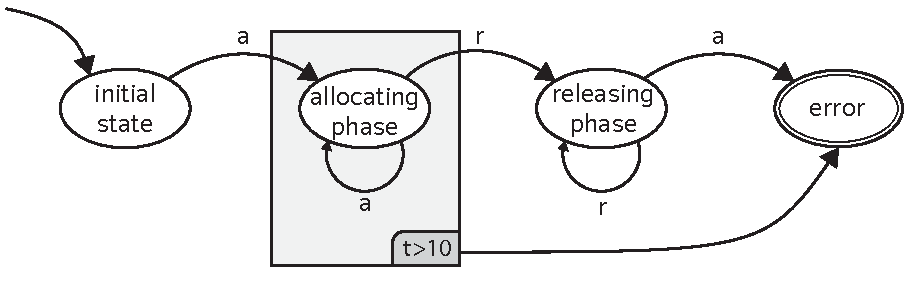
\includegraphics[width=0.7\linewidth]{figures/chapter_4/allocating_timed}
				\caption{Timed region event automaton of the two phase locking example \redraw}
				\label{fig:cep:trea}
			\end{figure}
			
			\subsection{Nondeterministic Timeout Event Automaton}
			
				For accepting languages generated by timed regular expressions, the concept of timed event automaton is introduced.	
				\todo{lost reference on \citep{alur1994theory}.}
				
				\begin{dfn}
					\label{dfn:cep:tea}
					A Nondeterministic Timeout Event Automaton is a tuple $\langle Q,\Sigma,\delta,q_0, F, C \rangle$ where
					\begin{itemize}
						\item $Q, \Sigma, q_0,$ and $F$ are the same as in \cref{dfn:cep:trea},	
						\item $C$ is a finite set of clocks.
						\item $\delta \subseteq \langle Q \times \Sigma' \times Q \times (\RR^+ \cup \{\infty\})^C \times 2^C \rangle$ i.e.~the transitions of the system in the order of:
							the state which is the source of the transition,
							the corresponding event for the transition (or $\varepsilon$ if it is an $\varepsilon$-transition),
							the state which is the destination of the transition,
							a function which assigns time values for each clock,
							and the set of clocks which needs to be reset upon firing the transition.
					\end{itemize}
				\end{dfn}
			
				\begin{dfn}
					\label{dfn:cep:tea:inputseq}
					A timed input sequence is denoted $(e_0, t_1, e_1, \dots, t_n, e_n)$ where $e_i \in \Sigma'$ and $t_i \in \RR^+_0$ i.e.~ a sequence of events and the elapsed times between them.
				\end{dfn}
			
				\begin{dfn}
				\label{dfn:cep:tea:trace}
				A trace in a Timeout Event Automaton is a sequence described as
				$(r_0, \langle a_1, t_1, v_1\rangle, \dots, \langle a_n, t_n, v_n \rangle, r_n)$, where $\forall r_i \in Q, \forall a_i \in \Sigma', \forall t_i \in \RR^+$ i.e.~a sequence of states, the elapsed time between them, and the clock assignments. The trace corresponds to to the timed input sequence $(e_0, t_1, e_1, \dots, t_n, e_n)$ if:
				\begin{itemize}
					\item $r_0 = q_0$, i.e.~the first state of the trace is the initial state of the Automaton,
					\item $\forall i \in [1,n - 1] \colon \langle r_i, a_{i+1}, r_{i+1}, u, \mathit{Res} \rangle \in \delta$,
						${v_i}' = v_i + t_{i+1}$, $\forall c \in C \colon {v_i}'(c) < u(c)$, and
						$$v_{i+1} = \begin{cases}
										0      & \text{if\ } c \in    \mathit{Res} \\
										{v_i}' & \text{if\ } c \notin \mathit{Res}
									\end{cases}$$
					\item The last $r_n$ is reached after reading the entire input sequence.	
				\end{itemize}
				A trace is accepting if $r_n \in F$.
				\end{dfn}
				
				\begin{dfn}
					\label{dfn:cep:tea:accepting}
					A Nondeterministic Timeout Event Automaton accepts a timed input sequence if exists an accepting trace for the timed input sequence.
				\end{dfn}
				
				\begin{dfn}
					\label{dfn:cep:tea:token}
					A token in a Nondeterministic Timeout Event Automaton is a set of the active states with their timer values.
				\end{dfn}
				
				The semantics of the timed deterministic finite automaton is defined as follows:
				
				\todo{Revision required}
				
				$Q_t \subseteq Q$ is the set of states with outgoing timed transitions, 
				i.e.~$\forall s \in Q_t$ : $ \exists t, t \in \delta \colon t = \langle s, a, s', h, c \rangle$, where $a \in \Sigma$, $s' \in Q$, $h \neq \emptyset$, and $c \neq \emptyset$.
				
				We have to define rules for entering states with timed outgoing transitions and we also define the general rules of changing states. 
				The current tokens in the automaton are noted as $\tau_{act}$.
				
				\begin{enumerate}
					\item Initialization rule: 
						$\forall c \in C \colon c \coloneqq \infty$, i.e.~on initialization of the automaton, all timeout clocks must be invalidated.
						On initialization a token must be placed on the initial state of the automaton.
					\item Firing Transitions Rule:
						$Q_{act}$ is the set of states which contains tokens.
						Upon receiving input $i$, where $i \in \Sigma$, $\forall q \in Q_{act}$, $\forall t \in \delta \colon \delta \langle q, i, q', T, \mathit{Res} \rangle$,
						$\forall c \in \mathit{Res} \colon c \coloneqq \infty$,
						$\forall c \in C \colon c \coloneqq T(c)$,
						the token is copied from $q$ to $q'$.
						The old tokens which are not created in this step must be removed.
					\item Timeout Rule:
						If one of the clocks reaches 0 for a token, the computation fails, and the token must be removed.
				\end{enumerate}
	
		\subsection{Transformation from Timed Regular Expressions to Timed Automata}
			\label{section:tre2tnfa}	
			Constructing a Timeout Region Automaton from a Timeout Regular expression depends on the steps described in \cref{section:re2nfa} as only one new operator has been added to the language.
			This operator can be compiled to a Nondeterministic Timeout Region Automaton as show on %\cref{Intentionally broken}. 
			.\todo{Draw this!}
			
			The timeout regions can be compiled into a \todo{Text}
		
			This construction yields an automaton with $\varepsilon$-transitions. Determinizing the nondeterministic automaton constructed from a timed regular expression is not a solved problem \emph{yet}. However, there are some results regarding the transformation from a subset of MTL to deterministic timed automaton~\citep{nivckovic2010mtl}.
			
			Testing whether a timed automaton is determinizable has been proved undecidable\citep{finkel2006undecidable}.
			Also, the undecidability of universality has been further investigated, and rather restricted classes of timed automata suffer from that undecidability result. On the other hand, classes of timed automata have been exhibited, that either can be effectively determinized (for instance event-clock timed automata \citep{alur1994determinizable}, or timed automata
			with integer resets \citep{suman2008timed}), or for which universality can be decided (for instance single-clock timed automata \citep{ouaknine2004language}).\citep{baier2009timed}.
			This means that we need further research in this direction, to find out whether nondeterministic timed region automatons generated from timed regular expressions can be determinized, or not.
			
	
	\section{Parametric Timed Languages}
	
			Complex systems usually have parametric behaviors, which can be expressed by formalisms extended with parameters. In this section we overview such formalisms that generate the parametric timed regular languages and an automaton formalism accepting them.
			
		\subsection{Parametric Timed Regular Expression}
		
		In this section I will overview the parametric extension of the Timed Regular Expression formalism.
			
			\begin{dfn}
				\label{dfn:cep:ptrea:event}
				A Parametric Event $\Gamma$ is a tuple $\langle \Sigma, P \rangle$, where 
				\begin{itemize}
					\item $\Sigma$ the input alphabet, as described formerly in \cref{dfn:cep:tre},
					\item and $P$ is a relation with the parameters. It describes that for the given event what are the parameter values. For a given event the size of $P$ must be the same.
				\end{itemize}
			\end{dfn}
			
	
			\begin{dfn}
			A Parametric Timed Regular Expression is a Timed Regular Expression as described in \cref{dfn:cep:tre}, but in this case we use $\Gamma$ instead of $\Sigma$.
			
%			timed regular expression where the set of events are defined as a set of tuples, $\langle \Sigma, P \rangle$,
%			where $\Sigma$ is defined as formerly and $P$ is a set of parameters.
			\end{dfn}
			
			With parametric timed regular expressions the example can be extended regular expression with parameters. \\
			$(a[i] a[i]^\ast  r[i] r[i]^\ast a[i]) | (\langle a[i] a[i]^\ast r[i]\rangle_{t > 10} )$ \\ \todo{Spacing}
			Note that this allows us to have only one instance of the automaton even for multiple tasks, each with its own ID.
		
		\subsection{Parametric Timed Region Event Automaton}
			
			\todo{Revision needed}
			

			\begin{dfn}
				\label{dfn:cep:ptrea}
				A Parametric Timed Region Event Automaton $\langle Q,\Gamma,\delta,q_0, F, t, T \rangle$ where
				\begin{itemize}
					\item $Q, \delta, q_0, F, t$ and  $T$ are the same as in \cref{dfn:cep:trea},
					\item $\Gamma$ is a finite, nonempty set, representing the parametric event set of the automaton.
				\end{itemize}
			\end{dfn}


			The semantics are only changed in the transition rules, described as:
			\begin{itemize}
				\item The transitions are only enabled if the fix parameters in the transition matches the event parameters. For example if the pattern contains $\dots \; a[i,2] \; \dots$, if an event $a$ occurs then the the second parameter must be $2$ to enable the transition for that event,
				\item A transition is enabled if the event parameters can be bound to the parameters of the token in the input location, and the corresponding tokens with the parameter bindings will be copied from the input to the output.
			\end{itemize}
	
			Using the parametric timed region automaton we can compile our timed regular expression 
			$(a[i] \; a[i]^\ast \; r[i] \; r[i]^\ast \; a[i]) | (\langle a[i] \; a[i]^\ast \; r[i]\rangle_{t > 10} )$ into the automaton on \cref{fig:cep:ptrea}.
	
	
			\begin{figure}[h]
			\centering
			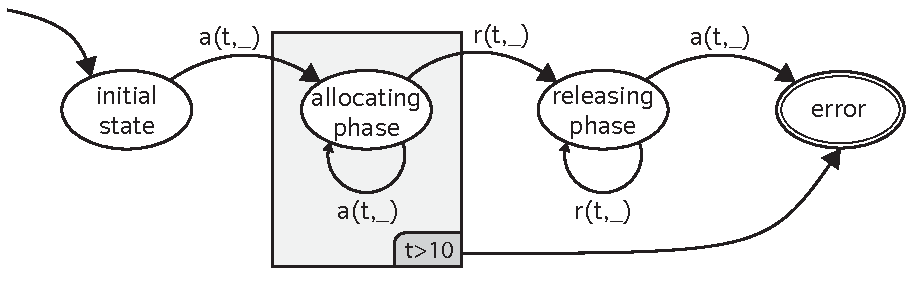
\includegraphics[width=0.7\linewidth]{figures/chapter_4/allocating_timed_parametric}
			\caption{Parametric timed region event automaton of the two phase locking example \redraw}
			\label{fig:cep:ptrea}
			\end{figure}
	
		\subsection{Parametric Timed Event Automaton}
		
		As in the case of the Timeout Region Event Automaton, the case is somewhat similar here; a formalism is introduced, swhich is more general and well-known in the literature. 
		
		\todo{Revision needed}
		
		\begin{dfn}
			\label{dfn:cep:ptea}
			A Nondeterministic Parametric Timeout Event Automaton is a tuple $\langle Q,\Gamma,\delta,q_0, F, C \rangle$ where
			\begin{itemize}
				\item $Q, \delta, q_0, F,$ and $C$ are the same as in \cref{dfn:cep:tea},	
				\item $\Gamma$ is a finite, nonempty set, representing the parametric event set of the automaton.
			\end{itemize}
		\end{dfn}
		
		\begin{dfn}
			\label{dfn:cep:ptea:inputseq}
			A timed parametric input sequence is denoted $(e_0, t_1, e_1, \dots, t_n, e_n)$ where $e_i \in \Gamma$ and $t_i \in \RR^+_0$ i.e.~ a sequence of parametric events and the elapsed times between them.
		\end{dfn}
		
		\begin{dfn}
			\label{dfn:cep:ptea:trace}

			A trace in a Parametric Timeout Event Automaton is a sequence
			$(r_0, \langle a_1, t_1, v_1\rangle, \dots, \langle a_n, t_n, v_n \rangle, r_n)$, where $\forall r_i \in Q, \forall a_i \in \Gamma, \forall t_i \in \RR^+$ i.e.~a sequence of states, the elapsed time between them, and the clock assignments. The trace corresponds to to the timed input sequence $(e_0, t_1, e_1, \dots, t_n, e_n)$ if:
			\begin{itemize}
				\item $r_0 = q_0$, i.e.~the first state of the trace is the initial state of the Automaton,
				\item $\forall i \in [1,n - 1] \colon \langle r_i, a_{i+1}, r_{i+1}, u, \mathit{Res} \rangle \in \delta$, 
				${v_i}' = v_i + t_{i+1}$, $\forall c \in C \colon {v_i}'(c) < u(c)$,\\
				$$v_{i+1} = \begin{cases}
				0      & \text{if\ } c \in    \mathit{Res} \\
				{v_i}' & \text{if\ } c \notin \mathit{Res}
				\end{cases}$$
				\item The last $r_n$ is reached after reading the entire input sequence.	
			\end{itemize}
			A trace is accepting if $r_n \in F$.
		\end{dfn}
		
		\begin{dfn}
			\label{dfn:cep:ptea:accepting}
			A Parametric Timeout Event Automaton accepts a timed input sequence if exists an accepting trace for the timed input sequence.
		\end{dfn}
		
		\begin{dfn}
			\label{dfn:cep:ptea:token}
			A token in a Parametric Timeout Event Automaton is a set of the active states with their timer values.
		\end{dfn}
		
		The semantics are changed as in the case of the Parametric Timeout Region Automaton.\todo{Ehunn egy link}
		
		\subsection{Transformation from Parametric Timed Regular Expression to Parametric Timed Event Automaton}
		\label{section:ptre2tnfa}	
			
		Constructing a Parametric Timeout Region Automaton from a Parametric Timeout Regular Expression depends on the steps described in \cref{section:tre2tnfa} as only the event has been parametrized. The transformation of the new events require some kind of auxiliary data structure be constructed which can determine that the a given event parameter on a given transition corresponds to which token parameter. For example, if the event $\dots \; a[i,j] \; \dots$ should be transformed, then this auxiliary data structure should contain, that for this transition event's first parameter the corresponding token parameter is $i$ and for the second parameter the corresponding token parameter is $j$. 
		
	
		Constructing a nondeterminsitic parametric timed region automaton from a parametric timed regular expression is possible according to the results know for timed regular expressions. As parametric automata are always nondeterminstic, thanks to the possibility of multiple tokens, we have no intention to determinize such automata.
		However, at least the $\varepsilon$-transitions should be eliminated from the automata, for the purpose of efficient execution, and analysis.
		
		To our best knowledge, there are no results about eliminating $\varepsilon$-transitions from a parametric time region automaton, being generated from parametric timed regular expression.
		